\section*{Đề kiểm tra Chương 4}
\subsection*{Đề số 1}
\setcounter{ex}{0}\setcounter{bt}{0}
\Opensolutionfile{ans}[ans/ans-KT-401]
\noindent\textbf{I. PHẦN TRẮC NGHIỆM}
\Opensolutionfile{ans}
\begin{ex}%[Lê Minh Thiện Anh, Dự án BG10-Lần2]%[0H1Y1-1]
	Véc-tơ có điểm đầu $E$, điểm cuối $F$ được kí hiệu là
	\choice
	{$FE$}
	{$\left|\overrightarrow{EF}\right|$}
	{$\overrightarrow{FE}$}
	{\True $\overrightarrow{EF}$}
	\loigiai
	{Véc-tơ có điểm đầu $E$, điểm cuối $F$ được kí hiệu là $\overrightarrow{EF}$}
\end{ex}

\begin{ex}%[Lê Minh Thiện Anh, Dự án BG10-Lần2]%[0H1Y1-3]
	Hai véc-tơ được gọi là bằng nhau khi và chỉ khi
	\choice
	{Giá của chúng trùng nhau và độ dài của chúng bằng nhau}
	{Chúng trùng với một trong các cặp cạnh đối của hình bình hành}
	{Chúng trùng với một trong các cặp cạnh của tam giác đều}
	{\True Chúng cùng hướng và có độ dài bằng nhau}
	\loigiai
	{Theo định nghĩa hai véc-tơ bằng nhau là hai véc-tơ có cùng hướng và độ dài bằng nhau.}
\end{ex}

\begin{ex}%[Lê Minh Thiện Anh, Dự án BG10-Lần2]%[0H1Y1-3]
	Cho hình bình hành $ABCD$, mệnh đề nào trong các mệnh đề sau đây là \textbf{đúng}?
	\choice
	{\True $\overrightarrow{AB}=\overrightarrow{DC}$}
	{$\overrightarrow{AD}=\overrightarrow{CB}$}
	{$\overrightarrow{CA}=\overrightarrow{DB}$}
	{$\overrightarrow{AB}=\overrightarrow{CD}$}
	\loigiai
	{Do $ABCD$ là hình bình hành nên $\overrightarrow{AB}=\overrightarrow{DC}$.
	\begin{center}
			\begin{tikzpicture}[scale=1, font=\footnotesize,line join=round, line cap=round, >=stealth]
			\coordinate (A) at (0,0);
			\coordinate (B) at (3,0);
			\coordinate (D) at (-1.5,-1);
			\coordinate (C) at ($(D)+(B)-(A)$);
			\tkzDrawPoints[fill=black](A,B,C,D)
			\draw (A)node[above]{$A$} -- (B)node[above]{$B$};
			\draw (C)node[below]{$C$} -- (D)node[below]{$D$} (B)--(C);
			\draw (A)--(C) (A)--(D) (B)--(D);
			\end{tikzpicture}
	\end{center}}
\end{ex}

\begin{ex}%[Lê Minh Thiện Anh, Dự án BG10-Lần2]%[0H1B2-4]
	Cho hình bình hành $ABCD$, khi đó $\overrightarrow{AB}-\overrightarrow{AC}$ bằng
	\choicefix
	{$\overrightarrow{BD}$}
	{\True $\overrightarrow{CB}$}
	{$\overrightarrow{0}$}
	{$\overrightarrow{BC}$}
	\loigiai
	{Theo quy tắc ba điểm ta có $\overrightarrow{AB}-\overrightarrow{AC}=\overrightarrow{CB}$.}
\end{ex}

\begin{ex}%[Lê Minh Thiện Anh, Dự án BG10-Lần2]%[0H1B1-1]
	Cho ba điểm phân biệt $M$, $N$, $P $ Có bao nhiêu vectơ khác vectơ không có điểm đầu và điểm cuối là các điểm $M$, $N$, $P$ đã cho?
	\choice
	{$5 $}
	{$4 $}
	{\True $6 $}
	{$8 $}
	\loigiai{Có $3$ đoạn thẳng phân biệt là $MN$, $NP$, $PM$ nên sẽ có $6$ véc tơ. }
\end{ex}

\begin{ex}%[Lê Minh Thiện Anh, Dự án BG10-Lần2]%[0H1B1-3]
	Cho hình bình hành $MNPQ$, khi đó
	\choice
	{$\overrightarrow{MN}=\overrightarrow{PQ}$ và $\overrightarrow{NP}=\overrightarrow{MQ}$}
	{$\overrightarrow{MN}=\overrightarrow{PQ}$ và $\overrightarrow{NP}=\overrightarrow{QM}$}
	{$\overrightarrow{MN}=\overrightarrow{QP}$ và $\overrightarrow{NP}=\overrightarrow{QM}$}
	{\True $\overrightarrow{MN}=\overrightarrow{QP}$ và $\overrightarrow{NP}=\overrightarrow{MQ}$}
	\loigiai
	{\immini
		{Do $MNPQ$ là hình bình hành nên $\overrightarrow{MN}=\overrightarrow{QP}$ và $\overrightarrow{NP}=\overrightarrow{MQ}$.}
		{\begin{tikzpicture}[scale=1, font=\footnotesize,line join=round, line cap=round, >=stealth]
			\coordinate (M) at (0,0);
			\coordinate (N) at (3,0);
			\coordinate (Q) at (-1.5,-1.5);
			\coordinate (P) at ($(Q)+(N)-(M)$);
			\tkzDrawPoints[fill=black](M,N,P,Q)
			\draw (M)node[above]{$M$} -- (N)node[above]{$N$};
			\draw (P)node[below]{$P$} -- (Q)node[below]{$Q$} (N)--(P) (M)--(Q);
			\end{tikzpicture}}}
\end{ex}

\begin{ex}%[Lê Minh Thiện Anh, Dự án BG10-Lần2]%[0H1Y2-4]
	Trong các mệnh đề sau đây, mệnh đề nào \textbf{sai}?
	\choice
	{Hai véc-tơ bằng nhau thì cùng phương}
	{Hai véc-tơ đối nhau thì cùng độ dài}
	{Hai véc-tơ cùng hướng thì cùng phương}
	{\True Hai véc-tơ cùng phương thì cùng hướng}
	\loigiai
	{Hai véc-tơ cùng phương thì cùng hướng hoặc ngược hướng.}
\end{ex}

\begin{ex}%[Lê Minh Thiện Anh, Dự án BG10-Lần2]%[0H1B2]
	Cho ba điểm phân biệt $A, B, C$. Khẳng định nào sau đây đúng?
	\choice
	{\True $\overrightarrow{AC}+\overrightarrow{BA}=\overrightarrow{BC}$}
	{$\overrightarrow{AC}+\overrightarrow{AB}=\overrightarrow{CB}$}
	{$\overrightarrow{AB}-\overrightarrow{BC}=\overrightarrow{CA}$}
	{$\overrightarrow{BA}-\overrightarrow{CA}=\overrightarrow{CB}$}
	\loigiai{Ta có $\overrightarrow{AC}+\overrightarrow{BA}=\overrightarrow{BA}+\overrightarrow{AC}=\overrightarrow{BC}$.
	}
\end{ex}

\begin{ex}%[Lê Minh Thiện Anh, Dự án BG10-Lần2]%[0H1B2]
	Cho hình bình hành $ABCD$. Khẳng định nào sau đây đúng?
	\choice
	{$\overrightarrow{AD}+\overrightarrow{BD}+\overrightarrow{CD}=\overrightarrow{0}$}
	{$\overrightarrow{CD}+\overrightarrow{CB}-\overrightarrow{AC}=\overrightarrow{0}$}
	{$\overrightarrow{BC}+\overrightarrow{DC}+\overrightarrow{AC}=\overrightarrow{0}$}
	{\True $\overrightarrow{AD}+\overrightarrow{AB}-\overrightarrow{AC}=\overrightarrow{0}$}
	\loigiai{Ta có $\overrightarrow{AD}+\overrightarrow{AB}=\overrightarrow{AC}$ nên $\overrightarrow{AD}+\overrightarrow{AB}-\overrightarrow{AC}=\overrightarrow{0}$.
	}
\end{ex}

\begin{ex}%[Lê Minh Thiện Anh, Dự án BG10-Lần2]%[0H1Y2-1]
	Khẳng định nào sau đây là {\bf sai}?
	\choice
	{\True Tổng của hai véc-tơ đối nhau bằng 0}
	{Véc-tơ-không cùng hướng với mọi véc-tơ}
	{Hai véc-tơ đối nhau là hai véc-tơ ngược hướng và cùng độ dài}
	{Hai véc-tơ cùng hướng thì chúng cùng phương}
	\loigiai{
		Tổng của hai véc-tơ đối nhau bằng véc-tơ-không.
	}
\end{ex}

\begin{ex}%[Lê Minh Thiện Anh, Dự án BG10-Lần2]%[0H1Y4-2]
	Cho hình bình hành $ABCD$ có $AD=2$ cm, $AB=4$ cm, $DB=5$ cm. Tính $\left|\overrightarrow{BA}-\overrightarrow{DA} \right| $.
	\choice
	{$3$ cm}
	{\True $5$ cm}
	{$4$ cm}
	{$6$ cm}
	\loigiai{
		Ta có $\left|\overrightarrow{BA}-\overrightarrow{DA} \right|= \left|\overrightarrow{BD}\right|=BD=5$ cm.		
	}
\end{ex}

\begin{ex}%[Lê Minh Thiện Anh, Dự án BG10-Lần2]%[0H1B2-1]
	Cho bốn điểm $A$, $B$, $C$, $D$ bất kì. Khi đó, véc-tơ $\overrightarrow{u}=\overrightarrow{DC}+\overrightarrow{AD}+\overrightarrow{BA}+\overrightarrow{CB}$ bằng véc-tơ nào sau đây?
	\choice
	{$\overrightarrow{u}=\overrightarrow{CD}$}
	{$\overrightarrow{u}=\overrightarrow{AC}$}
	{\True $\overrightarrow{u}=\overrightarrow{0}$}
	{$\overrightarrow{u}=\overrightarrow{AD}$}
	\loigiai{
		Ta có $\overrightarrow{u}=\overrightarrow{AD}+\overrightarrow{DC}+\overrightarrow{CB}+\overrightarrow{BA}=\overrightarrow{AC}+\overrightarrow{CA}=\overrightarrow{0}$.
	}
\end{ex}

\begin{ex}%[Lê Minh Thiện Anh, Dự án BG10-Lần2]%[0H1Y3-1]
	\immini
	{Cho ba điểm $A$, $M$, $B$ như hình vẽ.}
	{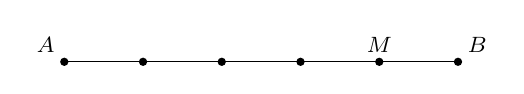
\begin{tikzpicture}[>=stealth,line join=round,line cap=round,font=\footnotesize,scale=1]
		\coordinate[label=above left:$A$] (A) at (0,0);
		\coordinate (C) at (1,0);
		\coordinate (D) at (2,0);
		\coordinate (E) at (3,0);
		\coordinate[label=above right:$B$] (B) at (5,0);
		\coordinate[label=above:$M$] (M) at (4,0);
		\draw (A)--(B);
		\fill (A) circle (1.5pt) (B) circle (1.5pt) (C) circle (1.5pt) (D) circle (1.5pt) (M) circle (1.5pt) (E) circle (1.5pt);
		\end{tikzpicture}}
	Khẳng định nào sau đây $\textbf{đúng}$?
	\choice
	{$\overrightarrow{MA}=-4\overrightarrow{MB}$}
	{\True $\overrightarrow{MA}=-3\overrightarrow{MB}$}
	{$\overrightarrow{MA}=3\overrightarrow{MB}$}
	{$\overrightarrow{MB}=-3\overrightarrow{MA}$}
	\loigiai{
		Nhìn vào hình vẽ ta có $MA=3MB$.\\
		Mà $\overrightarrow{MA}$ và $\overrightarrow{MB}$ ngược hướng.\\
		Vậy $\overrightarrow{MA}=-3\overrightarrow{MB}$.
	}
\end{ex}

\begin{ex}%[Lê Minh Thiện Anh, Dự án BG10-Lần2]%[0H1B3]
	Gọi $G$ là trọng tâm tam giác $ABC$. Đẳng thức nào sau đây đúng?
	\choice{$\overrightarrow{AG}= \dfrac{1}{2}\overrightarrow{AB}+ \dfrac{1}{2}\overrightarrow{AC} $}
	{\True $\overrightarrow{AG}= \dfrac{1}{3}\overrightarrow{AB}+ \dfrac{1}{3}\overrightarrow{AC} $}
	{$\overrightarrow{AG}= \dfrac{3}{2}\overrightarrow{AB}+ \dfrac{3}{2}\overrightarrow{AC} $}
	{$\overrightarrow{AG}= \dfrac{2}{3}\overrightarrow{AB}+ \dfrac{2}{3}\overrightarrow{AC} $}
	\loigiai{Gọi $M$ là trung điểm $BC$.
		Khi đó $ \overrightarrow{AM}= \dfrac{1}{2}\overrightarrow{AB}+ \dfrac{1}{2}\overrightarrow{AC}$.\\
		Mà $ \overrightarrow{AG}= \dfrac{2}{3}\overrightarrow{AM}$
		$ \Rightarrow \overrightarrow{AG}= \dfrac{1}{3}\overrightarrow{AB}+ \dfrac{1}{3}\overrightarrow{AC}$.}
\end{ex}

\begin{ex}%[Lê Minh Thiện Anh, Dự án BG10-Lần2]%[0H1Y3-2]
	Cho tam giác $ABC$ có đường trung tuyến $AM$ và trọng tâm $G$. Đẳng thức nào sau đây là đúng?
	\choice
	{\True $\overrightarrow{GA}=-\dfrac{2}{3}\overrightarrow{AM}$}
	{$\overrightarrow{GA}=2\overrightarrow{GM}$}
	{$\overrightarrow{GA}=\dfrac{2}{3}\overrightarrow{GM}$}
	{$\overrightarrow{GA}=\dfrac{1}{2}\overrightarrow{AM}$}
	\loigiai{
		\immini{
			Từ tính chất của trọng tâm, ta có $\overrightarrow{GA}=-\dfrac{2}{3}\overrightarrow{AM}$.
		}{
			\begin{tikzpicture}[line cap=round, line join= round, font=\footnotesize,>=stealth,scale=1]
			\tkzDefPoints{0/0/B,3/0/C,1/2/A}
			\tkzDefMidPoint(B,C)\tkzGetPoint{M}
			\path ($(A)!2/3!(M)$) coordinate (G);
			\draw (A)--(B)--(C)--cycle
			(A)--(M);
			\foreach \x/\y in {A/100,B/-135,C/-45,M/-90,G/-160} \draw[fill=black] (\x) circle (1pt)+(\y:0.3) node{$\x$};
			\end{tikzpicture}
		}	
	}
\end{ex}

\begin{ex}%[Lê Minh Thiện Anh, Dự án BG10-Lần2]%[0H1Y3-2]
	Điều kiện cần và đủ để điểm $O$ là trung điểm của đoạn $AB$ là
	\choice
	{$OA=OB$}
	{$\overrightarrow{OA}= \overrightarrow{OB}$}
	{$\overrightarrow{AO}= \overrightarrow{BO}$}
	{\True $\overrightarrow{OA}+ \overrightarrow{OB}= \overrightarrow{0}$}
	\loigiai
	{
		Điều kiện cần và đủ để điểm $O$ là trung điểm của đoạn $AB$ là $\overrightarrow{OA}+ \overrightarrow{OB}=\overrightarrow{0}$.
	}
\end{ex}

\begin{ex}%[Lê Minh Thiện Anh, Dự án BG10-Lần2]%[0H1B3-1]
	Trên đoạn thẳng $A B$, lấy điểm $M$ sao cho $A B=3 A M$ như hình vẽ sau:
	\begin{center}
		\begin{tikzpicture}[>=stealth,line join=round,line cap=round,font=\footnotesize,scale=1]
		\coordinate[label=below left:$A$](A) at (0,0);
		\coordinate[label=below right:$B$](B) at (6,0);
		\coordinate[label = below:$M$] (M) at ($(A)!1/3!(B)$);
		\draw (A)--(B);
		\fill[black] (A) circle (1.5pt) (B) circle (1.5pt) (M) circle (1.5pt);
		\end{tikzpicture}
	\end{center}
	Mệnh đề nào sau đây đúng?
	\choice
	{$\overrightarrow{M B}=2 \overrightarrow{M A}$}
	{$\overrightarrow{M A}=2 \overrightarrow{M B}$}
	{\True $\overrightarrow{M B}=-2 \overrightarrow{M A}$}
	{$\overrightarrow{M A}=-2 \overrightarrow{M B}$}
	\loigiai{
		Dựa vào giả thiết và hình vẽ ta có $\overrightarrow{M B}=-2 \overrightarrow{M A}$.
	}
\end{ex}

\begin{ex}%[Lê Minh Thiện Anh, Dự án BG10-Lần2]%[0H1Y4-3]
	Trong hệ tọa độ $Oxy$, cho $A(2;6)$, $B(8;-2)$. Tọa độ trung điểm của đoạn thẳng $AB$ là
	\choice
	{$(3;-4)$}
	{$(5;-2)$}
	{$(5;-4)$}
	{\True $(5;2)$}
	\loigiai
	{
		Gọi $M(x_M;y_M)$ là trung điểm của đoạn thẳng $AB$.\\
		Ta có
		\[\left\{\begin{aligned}&x_M=\dfrac{x_A+x_B}{2} \\&y_M=\dfrac{y_A+y_B}{2}\end{aligned}\right. \Leftrightarrow \left\{\begin{aligned}&x_M=\dfrac{2+8}{2} \\&y_M=\dfrac{6-2}{2}\end{aligned}\right. \Leftrightarrow \left\{\begin{aligned}&x_M=5 \\&y_M=2.\end{aligned}\right.\]
		Vậy $M(5;2)$ là trung điểm của đoạn thẳng $AB$.
	}
\end{ex}

\begin{ex}%[Lê Minh Thiện Anh, Dự án BG10-Lần2]%[0H1Y4-3]
	Trong mặt phẳng tọa độ $Oxy$, cho $\overrightarrow{OA}=2\overrightarrow{i}-3\overrightarrow{j}$. Tìm tọa độ điểm $A$.
	\choice
	{$A(2;3) $}
	{$A\left(2\overrightarrow{i};-3\overrightarrow{j}\right) $}
	{\True $A(2;-3) $}
	{$A(-2;3) $}
	\loigiai{
		Ta có $A(2;-3)$.
	}
\end{ex}

\begin{ex}%[Lê Minh Thiện Anh, Dự án BG10-Lần2]%[0H1B4-1]
	Trong mặt phẳng với hệ toạ độ $Oxy$, hình chiếu của điểm $M(3;5)$ trên trục hoành là điểm nào sau đây?
	\choice
	{$P(0;3)$}
	{$R(0;5)$}
	{$Q(5;0)$}
	{\True $N(3;0)$}
	\loigiai{
		Hình chiếu của điểm $M(3;5)$ trên trục hoành là $N(3;0)$.}
\end{ex}

\begin{ex}%[Lê Minh Thiện Anh, Dự án BG10-Lần2]%[0H1Y4-3]
	Trong mặt phẳng $Oxy$, cho $A(1;3)$, $B(2;-5)$. Tìm tọa độ của véc-tơ $\overrightarrow{AB}$.
	\choice
	{$\overrightarrow{AB}=(3;-2)$}
	{\True $\overrightarrow{AB}=(1;-8)$}
	{$\overrightarrow{AB}=(2;-15)$}
	{$\overrightarrow{AB}=(-1;8)$}
	\loigiai{
		Tọa độ $\overrightarrow{AB}=(1;-8)$.	
	}
\end{ex}

\begin{ex}%[Lê Minh Thiện Anh, Dự án BG10-Lần2]%[0H1B4-3]
	Cho hai điểm $A(1;0)$, $B(3;-2)$. Tọa độ trung điểm của đoạn thẳng $AB$ là
	\choice
	{$(2;-2)$}
	{\True $(2;-1)$}
	{$(-2;2)$}
	{$(-1;2)$}
	\loigiai{
		Gọi $I(x;y)$ là trung điểm $AB$. Suy ra $\heva{& x=\dfrac{1+3}{2}=2 \\ & y=\dfrac{0-2}{2}=-1}\Rightarrow I(2;-1)$.
	}
\end{ex}

\begin{ex}%[Lê Minh Thiện Anh, Dự án BG10-Lần2]%[0H1Y4-2]
	Trong mặt phẳng tọa độ $Oxy$, cho $\overrightarrow{a}=(2;-4)$; $\overrightarrow{b}=(-5;3)$. Tọa độ của $\overrightarrow{u}=2\overrightarrow{a}-\overrightarrow{b}$ là  
	\choice
	{\True $(9;-11)$}
	{$(9;11)$}
	{$(-9;11)$}
	{$(7;-7)$}
	\loigiai{
		Ta có\\
		$2\overrightarrow{a}=(4;-8)$\\
		$-\overrightarrow{b}=(5;-3)$\\
		Vậy $\overrightarrow{u}=2\overrightarrow{a}-\overrightarrow{b}=(9;-11)$.
	}
\end{ex}

\begin{ex}%[Lê Minh Thiện Anh, Dự án BG10-Lần2]%[0H1Y4-1]
	Trong mặt phẳng tọa độ $Oxy$, cho $A(1;1)$, $B(2;2)$. Tính độ dài đoạn thẳng $AB$.
	\choice
	{\True $\sqrt{2}$}
	{$0$}
	{$2$}
	{$3\sqrt{2}$}
	\loigiai{
		Với $A(1;1)$, $B(2;2)$ ta có $AB=\sqrt{(2-1)^2+(2-1)^2}=\sqrt{2}$.}
\end{ex}

\begin{ex}%[Lê Minh Thiện Anh, Dự án BG10-Lần2]%[0H2Y2-1]
	Trong mặt phẳng toạ độ $Oxy$ cho hai điểm $A(3;-1)$, $B(2;10)$. Tích vô hướng $\overrightarrow{OA}\cdot\overrightarrow{OB}$ bằng bao nhiêu?
	\choice
	{$0$}
	{\True $-4$}
	{$4$}
	{$16$}
	\loigiai{
		Ta có $\overrightarrow{OA}=(3;-1)$, $\overrightarrow{OB}=(2;10)$.\\
		Vậy $\overrightarrow{OA}\cdot\overrightarrow{OB}=-4$.
	}
\end{ex}

\begin{ex}%[Lê Minh Thiện Anh, Dự án BG10-Lần2]%[0H2B2-1]
	Cho hình vuông $ABCD$ có độ dài bằng $10$. Tính giá trị của $\overrightarrow{AB}\cdot \overrightarrow{CD}$.
	\choice
	{$100 $}
	{$10 $}
	{$0 $}
	{\True $-100 $}
	\loigiai{
	\immini{Ta có $\overrightarrow{AB}\cdot \overrightarrow{CD}=AB\cdot CD\cdot \cos\left(\overrightarrow{AB},\overrightarrow{CD}\right)=10\cdot 10\cdot \cos180^\circ=-10^2=-100$.}{\begin{tikzpicture}[line join = round, line cap = round,>=stealth,font=\footnotesize,scale=0.7]
			\tkzDefPoints{0/0/A}
			\coordinate (B) at ($(A)+(4,0)$);
			\tkzDefSquare(B,A)    \tkzGetPoints{D}{C}
			%
			\pgfresetboundingbox
			\tkzDrawPolygon(A,B,C,D)
			\tkzDrawPoints[fill=black](A,B,D,C)
			\tkzLabelPoints[above](A,B)
			\tkzLabelPoints[below](C,D)
	\end{tikzpicture}}
	}
\end{ex}

\begin{ex}%[Lê Minh Thiện Anh, Dự án BG10-Lần2]%[0H2B2-1]
Cho tam giác đều $ABC$ cạnh $a$. Khi đó tích vô hướng của hai vectơ $\overrightarrow{AB}\cdot\overrightarrow{AC}$ bằng
\choice
{\True $\dfrac{a^2}{2}$}
{$-a^2$}
{$a^2$}
{$-\dfrac{a^2}{2}$}
\loigiai{
	Ta có $\overrightarrow{AB}\cdot\overrightarrow{AC}=a\cdot a\cdot\cos 60^\circ=\dfrac{a^2}{2}$.
}
\end{ex}

\begin{ex}%[Lê Minh Thiện Anh, Dự án BG10-Lần2]%[0H2Y2-1]
	Trong mặt phẳng $Oxy$ cho hai véc-tơ $\overrightarrow{a}$ và $\overrightarrow{b}$ biết $\overrightarrow{a}=(1;-2)$, $\overrightarrow{b}=(-1;-3)$. Tính góc giữa hai véc-tơ $\overrightarrow{a}$ và $\overrightarrow{b}$
	\choice
	{$60^\circ$}
	{$30^\circ$}
	{$135^\circ$}
	{\True $45^\circ$}
	\loigiai{
		Ta có $\cos (\overrightarrow{a},\overrightarrow{b})=\dfrac{\overrightarrow{a}\cdot\overrightarrow{b}}{\left| \overrightarrow{a}\right| \cdot \left| \overrightarrow{b}\right|}=\dfrac{1\cdot (-1)+(-2)\cdot (-3)}{\sqrt{1^2+(-2)^2}\cdot\sqrt{(-1)^2+(-3)^2}}=\dfrac{1}{\sqrt{2}}$.\\
		Vậy $(\overrightarrow{a},\overrightarrow{b})=45^\circ$.
	}
\end{ex}

\begin{ex}%[Lê Minh Thiện Anh, Dự án BG10-Lần2]%[0H1Y4-2]
	Trong mặt phẳng tọa độ $Oxy$, cho $\overrightarrow{a}=(2;-5)$, $\overrightarrow{b}=(-1;2)$. Tính $\overrightarrow{a}+\overrightarrow{b}$.
	\choice
	{$(-1;3)$}
	{$(1;-7)$}
	{$(3;-3)$}
	{\True $(1;-3)$}
	\loigiai{
		Ta có $\overrightarrow{a}+\overrightarrow{b}=\left(2+(-1);(-5)+2\right)=(1;-3)$.
	}
\end{ex}

\begin{ex}%[Lê Minh Thiện Anh, Dự án BG10-Lần2]%[0H1Y4-2]
	Trong hệ trục tọa độ $Oxy$, cho hai điểm $M(1;1)$, $N(4;-1)$. Tính độ dài véc-tơ $\overrightarrow{MN}$.
	\choice
	{\True $\left|\overrightarrow{MN}\right|=\sqrt{13}$}
	{$\left|\overrightarrow{MN}\right|=5$}
	{$\left|\overrightarrow{MN}\right|=\sqrt{29}$}
	{$\left|\overrightarrow{MN}\right|=3$}
	\loigiai
	{
		Ta có $\overrightarrow{MN}=(3;-2) \Rightarrow \left|\overrightarrow{MN}\right|=\sqrt{3^2+\left(-2\right)^2}=\sqrt{13}$.
	}
\end{ex}

\begin{ex}%[Lê Minh Thiện Anh, Dự án BG10-Lần2]%[0H2B2-1]
	Trong mặt phẳng $(Oxy)$, các điểm $A(1 ; 1), B(2 ; 4)$ và $C(10 ;-2)$. Tính tích vô hướng $\overrightarrow{AB} \cdot \overrightarrow{AC}$.
	\choice
	{\True $0$}
	{$10$}
	{$-10$}
	{$-20$}
	\loigiai{
	Ta có: 	$\overrightarrow{AB}=(1;3); \overrightarrow{AC}=(9;-3)\Rightarrow \overrightarrow{AB} \cdot \overrightarrow{AC} =1\cdot 9+ 3\cdot(-3)=0$.
	}
\end{ex}

\begin{ex}%[Lê Minh Thiện Anh, Dự án BG10-Lần2]%[0H2B2-3]
	Cho hai véc-tơ $\overrightarrow{u}=(4;5)$ và $\overrightarrow{v}=(3;a)$. Tìm $a$ để $\overrightarrow{u}\cdot\overrightarrow{v}=0$.
	\choice
	{\True $a=-\dfrac{12}{5}$}
	{$a=\dfrac{12}{5}$}
	{$a=\dfrac{5}{12}$}
	{$a=-\dfrac{5}{12}$}
	\loigiai{
		Ta có $\overrightarrow{u}\cdot\overrightarrow{v}=0\Leftrightarrow 12+5a=0\Leftrightarrow a=-\dfrac{12}{5}$.
	}
\end{ex}

\begin{ex}%[Lê Minh Thiện Anh, Dự án BG10-Lần2]%[0H2Y2-1]
\immini{Gọi $R$ là trung điểm cạnh $MN$ của tam giác đều $MNQ$. Xác định góc giữa $\overrightarrow{NR}$ và $\overrightarrow{NQ}$.
	\choice
	{$0^\circ$}
	{\True $60^\circ$}
	{$120^\circ$}
	{$90^\circ$}
}
{
\begin{tikzpicture}[>=stealth,line join=round,line cap=round,font=\footnotesize,scale=1]
\path
(0,0)coordinate (Q)++(0:3)coordinate(N)++(120:1.5)coordinate(R)++(120:1.5)coordinate(M)
;
\draw (M)--(N)--(Q)--cycle;
\draw[->] (N)--(R);
\draw[->] (N)--(Q);
\foreach \x/\g in{M/90,N/0,R/45,Q/180}
\fill[black](\x)circle(1pt) ($(\x)+(\g:3mm)$)node{$\x$};	
\end{tikzpicture}	
}
	\loigiai{
	Góc giữa hai véc-tơ $\overrightarrow{NR}$ và $\overrightarrow{NQ}$ là $\widehat{QNR}=60^\circ$.
	}
\end{ex}

\begin{ex}%[Lê Minh Thiện Anh, Dự án BG10-Lần2]%[0H2B2-1]
Cho hình vuông $ABCD$ cạnh $a$. Khi đó $\overrightarrow{AB}\cdot\overrightarrow{AC}$ bằng
\choice
{$a^2\sqrt{2}$}
{$\dfrac{1}{2}a^2$}
{$\dfrac{\sqrt{2}}{2}a^2$}
{\True $a^2$}
\loigiai{
\immini{Cách 1\\
$\overrightarrow{AB}\cdot \overrightarrow{AC}=AB\cdot AC\cdot \cos45^\circ=a\cdot a\sqrt{2}\cdot\dfrac{\sqrt{2}}{2}=a^2$.\\
Cách 2\\
$\overrightarrow{AB}\cdot\overrightarrow{AC}=\overrightarrow{AB}\left(\overrightarrow{AB}+\overrightarrow{BC}\right)=\overrightarrow{AB}\cdot\overrightarrow{AB}+\overrightarrow{AB}\cdot\overrightarrow{BC}=AB^2=a^2$}{
\begin{tikzpicture}[scale=1,font=\footnotesize,line join = round, line cap = round, >= stealth]
\def\x{2.5}
\coordinate (A) at (0,0);
\coordinate (B) at (0:\x);
\coordinate (D) at (90:\x);
\coordinate (C) at ($(B)+(D)-(A)$);
\draw (A)--(B)--(C)--(D)--cycle;
\foreach \p/\g in {A/-90,B/-90,C/90,D/90} \draw[fill] (\p) circle(.5pt) node [shift={(\g:.3)}] {$\p$};
\end{tikzpicture}
}}
\end{ex}

\begin{ex}%[Lê Minh Thiện Anh, Dự án BG10-Lần2]%[0H2B2-1]
	 Cho các điểm $A(1;2)$, $B(-1;1)$, $C(5;-1)$. Giá trị $\cos\left(\overrightarrow{AB};\overrightarrow{AC}\right)$ bằng
	\choice
	{$\dfrac{\sqrt{5}}{5}$}
	{$\dfrac{2-1}{2}$}	
	{$\dfrac{\sqrt{3}}{2}$}
	{\True$\dfrac{-\sqrt{5}}{5}$}
	\loigiai{
		Ta có $\overrightarrow{AB}=(-2;-1)$,$\overrightarrow{AC}=(4;-3).\\$
		Khi đó $\cos\left(\overrightarrow{AB};\overrightarrow{AC}\right)=\dfrac{\overrightarrow{AB}\cdot\overrightarrow{AC}}{\left|\overrightarrow{AB}\right|\cdot\left|\overrightarrow{AC}\right|}=\dfrac{-2\cdot4+(-1)\cdot(-3)}{\sqrt{(-2)^2+(-1)^2}\cdot\sqrt{4^2+(-3)^2}}=-\dfrac{\sqrt{5}}{5}$.}
\end{ex}


\noindent\textbf{II. PHẦN TỰ LUẬN}
\begin{bt}%[Lê Minh Thiện Anh, Dự án BG10-Lần2]%[0H1K3-2]
	Cho $\triangle ABC$. Gọi $M$ là trung điểm của $AB$ và $N$ là một điểm trên cạnh $AC$ sao cho $NC=2NA$. Gọi $K$, $D$ lần lượt là trung điểm của $MN$ và $BC$. Chứng minh rằng
	\begin{enumerate}
		\item $\overrightarrow{AK}=\dfrac{1}{4}\overrightarrow{AB}+\dfrac{1}{6}\overrightarrow{AC}$.
		\item $\overrightarrow{KD}=\dfrac{1}{4}\overrightarrow{AB}+\dfrac{1}{3}\overrightarrow{AC}$.
	\end{enumerate}
	\loigiai{
		\begin{enumerate}
			\item \immini{Từ giả thiết $M$ là trung điểm của $AB$ và $N$ là một điểm trên cạnh $AC$ và $NC=2NA$ nên ta có $\overrightarrow{AM}=\dfrac{1}{2}\overrightarrow{AB}$ và $\overrightarrow{AN}=\dfrac{1}{3}\overrightarrow{AC}$.\\
				Vì $K$ là trung điểm của $MN$ nên theo tính chất trung điểm ta có $$\overrightarrow{AK}=\dfrac{1}{2}\overrightarrow{AM}+\dfrac{1}{2}\overrightarrow{AM}.$$
				Từ đó suy ra $\overrightarrow{AK}=\dfrac{1}{4}\overrightarrow{AB}+\dfrac{1}{6}\overrightarrow{AC}$.}{\begin{tikzpicture}[scale=0.8]
				\tkzDefPoints{3/5/A,1/0/B,7/0/C}
				\tkzDefMidPoint(B,A)\tkzGetPoint{M}
				\tkzDefPointBy[homothety = center A ratio 0.33](C)\tkzGetPoint{N}
				\tkzDefMidPoint(M,N)\tkzGetPoint{K}
				\tkzDefMidPoint(B,C)\tkzGetPoint{D}
				\tkzDrawSegments(A,B B,C C,A A,K K,D M,N)
				\tkzDrawPoints(A,B,C,N,M,K,D)
				\tkzLabelPoints[left](B,M)
				\tkzLabelPoints[right](N,C)
				\tkzLabelPoints[above](A)
				\tkzLabelPoints[below](D)
				\tkzLabelPoints[below right](K)
				\end{tikzpicture}}
			\item Vì $D$ là trung điểm của $BC$ nên ta có $\overrightarrow{AD}=\dfrac{1}{2}\overrightarrow{AB}+\dfrac{1}{2}\overrightarrow{AC}$.\\
			Mà $\overrightarrow{KD}=\overrightarrow{KA}+\overrightarrow{AD}=-\overrightarrow{AK}+\overrightarrow{AD}$. Từ đó theo chứng minh trên ta suy ra
			$$\overrightarrow{KD}=-\dfrac{1}{4}\overrightarrow{AB}-\dfrac{1}{6}\overrightarrow{AC}+\dfrac{1}{2}\overrightarrow{AB}+\dfrac{1}{2}\overrightarrow{AC}=\dfrac{1}{4}\overrightarrow{AB}+\dfrac{1}{3}\overrightarrow{AC}.$$	
		\end{enumerate}
	}
\end{bt}

\begin{bt}%[Lê Minh Thiện Anh, Dự án BG10-Lần2]%[0H1K4-5]  
	Trong mặt phẳng $Oxy$, cho các điểm $A(4;2)$, $B(-2;1 )$, $C(0;3)$, $M(-3;7)$. Tìm tọa độ điểm $N$ thuộc trục hoành để $NA+NB$ nhỏ nhất.
	\loigiai{
		Ta có $A(4;2)$, $B(-2;1)$ nên điểm $A$, $B$ nằm phía trên trục hoành vì có tung độ dương.\\
		Gọi $A'$ là điểm đối xứng với $A$ qua trục hoành $\Rightarrow A'( 4;-2 )$.\\
		Tổng $NA+NB=NA'+NB \ge A'B$.\\
		Đẳng thức xảy ra khi 3 điểm $A'$, $B$, $N$ thẳng hàng.\\
		Giả sử $N(n;0) \in Ox$ ta có $\overrightarrow{BA'}=(6;-3)$, $\overrightarrow{BN}=(n+2;-1)$.\\
		Các điểm $A'$, $B$, $N$ thẳng hàng $\Leftrightarrow \overrightarrow{BA'}$, $\overrightarrow{BN}$ cùng phương $\Leftrightarrow n=0 \Rightarrow N(0;0)$.\\
		Vậy $N(0;0)$.
	}
\end{bt}


\begin{bt}%[Lê Minh Thiện Anh, Dự án BG10-Lần2]%[0H2G2-5]
	Trong mặt phẳng $Oxy$, cho tam giác $ABC$ biết $A(1;3)$, $B(2;1)$, $C(-1;1)$. Tìm tọa độ điểm $M$ trên $BC$ sao cho $MA^2+MB^2+MC^2$ đạt giá trị nhỏ nhất. 	
\loigiai{
	Tọa độ trọng tâm $G$ của tam giác $ABC$ là $G\left(\dfrac{2}{3};\dfrac{5}{3}\right)$. Ta có 
	\begin{eqnarray*}
		MA^2+MB^2+MC^2&=&\overrightarrow{MA}^2+\overrightarrow{MB}^2+\overrightarrow{MC}^2\\
		&=&\left(\overrightarrow{MG}+\overrightarrow{GA}\right)^2+\left(\overrightarrow{MG}+\overrightarrow{GB}\right)^2+\left(\overrightarrow{MG}+\overrightarrow{GC}\right)^2 \\
		&=& 3\overrightarrow{MG}^2+\overrightarrow{GA}^2+\overrightarrow{GB}^2+\overrightarrow{GC}^2+2\overrightarrow{MG}\cdot\left(\overrightarrow{GA}+\overrightarrow{GB}+\overrightarrow{GC}\right)\\
		&=& 3MG^2+GA^2+GB^2+GC^2+2\overrightarrow{MG}\cdot\overrightarrow{0}\\
		&=& 3MG^2+GA^2+GB^2+GC^2.
	\end{eqnarray*}	
Do đó $MA^2+MB^2+MC^2$ đạt giá trị nhỏ nhất khi và chỉ khi độ dài đoạn thẳng $MG$ ngắn nhất. Khi đó điểm $M$ là hình chiếu vuông góc của $G$ trên đường thẳng $BC$.\\
Gọi $M(x;y)$, ta có $\overrightarrow{BC}=(-3;0)$, $\overrightarrow{BM}=\left(x-2;y-1\right)$ và $\overrightarrow{GM}=\left(x-\dfrac{2}{3};y-\dfrac{5}{3}\right)$.\\
Điểm $M$ là hình chiếu vuông góc của $G$ trên đường thẳng $BC$ khi và chỉ khi
\[\overrightarrow{GM}\cdot \overrightarrow{BC}=0\Leftrightarrow (-3)\cdot \left(x-\dfrac{2}{3}\right)+0\cdot \left(y-\dfrac{5}{3}\right)\Leftrightarrow x=\dfrac{2}{3}.\]
Suy ra $\overrightarrow{BM}=\left(-\dfrac{4}{3};y-1\right)$.\\
Vì $M\in BC$ nên $\overrightarrow{BM}$ và $\overrightarrow{BC}$ cùng phương, do đó
\[\heva{&-\dfrac{4}{3}=k\cdot(-3)\\&y-1=k\cdot 0}\Rightarrow y=1.\]
Vậy $M\left(\dfrac{2}{3};1\right)$.
	}	
\end{bt}
\Closesolutionfile{ans}
\Closesolutionfile{ansbook}
% \indapan{10}{ans/ans-KT-401}
